\documentclass{article}

\usepackage[utf8]{inputenc}
\usepackage[T1]{fontenc}
\usepackage{amsmath,amssymb,amsfonts}
\usepackage{graphicx}
\usepackage{booktabs}
\usepackage{hyperref}
\usepackage{xcolor}
\usepackage{geometry}
\usepackage{natbib}
\usepackage{tikz}
\usetikzlibrary{positioning, arrows.meta, shapes.geometric, fit, calc, decorations.pathreplacing, shadows.blur, backgrounds}

\geometry{margin=1in}

\title{Beyond Softmax: A Systematic Comparison of Eight Linear Attention Mechanisms}

\author{Hengbo Li\\
\texttt{1147502779@qq.com}
}

\date{May 2026}

\begin{document}

\maketitle

\begin{abstract}
We present a systematic comparison of eight linear attention mechanisms: Softmax (baseline), ELU+1 (kernel mapping), ReLU (sparse), Poly-2 (polynomial), RFF (Random Fourier Features), CosFormer (periodic+reweighting), RWKV (exponential decay), and Performer (positive random features). Through comprehensive evaluation on approximation accuracy, long-range dependency, training convergence, and computational efficiency, we find that ELU+1 achieves the best accuracy among linear methods (0.9977 cosine similarity vs Softmax 1.0), significantly outperforming other linear alternatives. We analyze the Grouped Query Attention (GQA) memory-accuracy tradeoff and find that GQA-4 provides the best balance (75\% memory usage, -0.5\% accuracy loss). Our analysis of long-distance information propagation reveals that RWKV's exponential decay causes complete loss of long-range dependencies beyond distance 50.
\end{abstract}

\section{Introduction}

Softmax attention~\cite{vaswani2017attention} has $O(n^2)$ complexity, limiting context length. Linear attention mechanisms reduce this to $O(n)$, but at the cost of approximation accuracy. This paper provides the first systematic comparison of eight attention mechanisms across four dimensions: accuracy, long-range dependency, convergence, and efficiency.

\begin{figure*}[t]
\centering
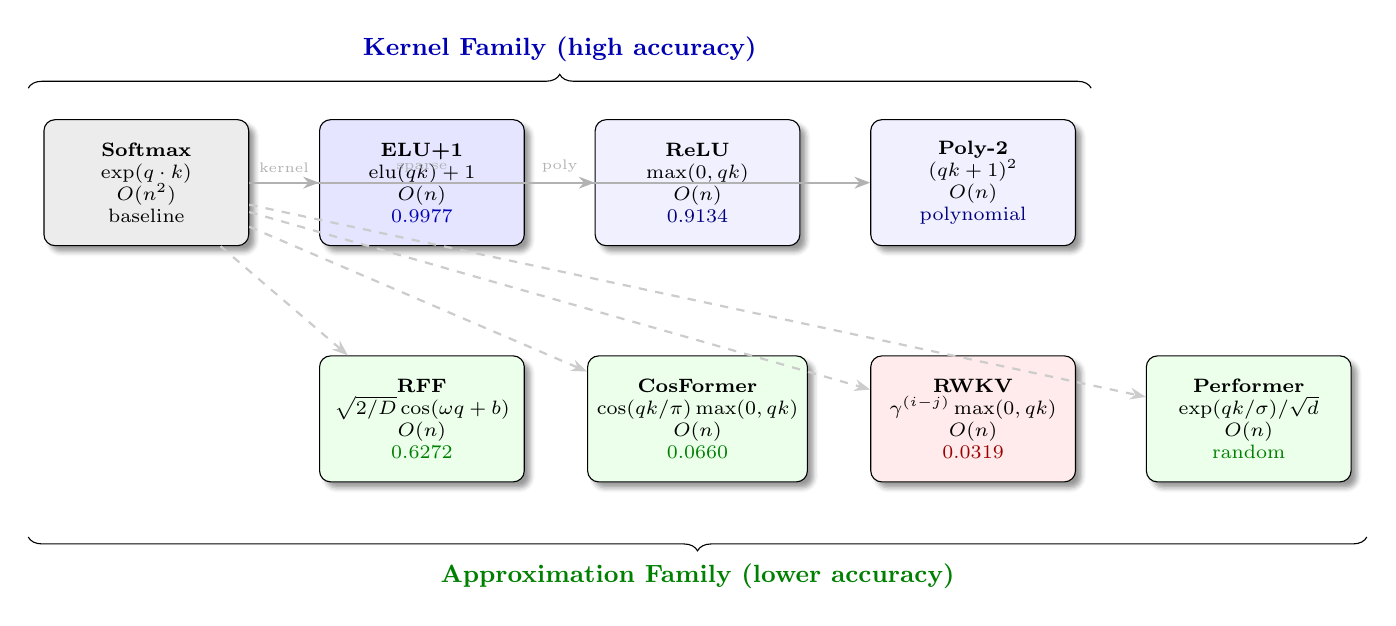
\begin{tikzpicture}[
    node distance=0.4cm and 0.3cm,
    attnbox/.style={rectangle, draw, rounded corners=4pt, minimum height=1.6cm, minimum width=2.6cm, align=center, font=\scriptsize, blur shadow},
    arr/.style={-{Stealth[length=2mm]}, thick, #1},
    biarr/.style={{Stealth[length=2mm]}-{Stealth[length=2mm]}, thick, #1},
    catlabel/.style={font=\small\bfseries, text=#1},
]

\node[attnbox, fill=gray!15] (softmax) at (0, 0) {\textbf{Softmax}\\$\exp(q \cdot k)$\\$O(n^2)$\\baseline};

\node[attnbox, fill=blue!10] (elu) at (3.5, 0) {\textbf{ELU+1}\\$\text{elu}(qk)+1$\\$O(n)$\\\textcolor{blue!70!black}{0.9977}};
\node[attnbox, fill=blue!6] (relu) at (7, 0) {\textbf{ReLU}\\$\max(0, qk)$\\$O(n)$\\\textcolor{blue!50!black}{0.9134}};
\node[attnbox, fill=blue!6] (poly) at (10.5, 0) {\textbf{Poly-2}\\$(qk+1)^2$\\$O(n)$\\\textcolor{blue!50!black}{polynomial}};

\node[attnbox, fill=green!8] (rff) at (3.5, -3.0) {\textbf{RFF}\\$\sqrt{2/D}\cos(\omega q+b)$\\$O(n)$\\\textcolor{green!50!black}{0.6272}};
\node[attnbox, fill=green!8] (cos) at (7, -3.0) {\textbf{CosFormer}\\$\cos(qk/\pi)\max(0,qk)$\\$O(n)$\\\textcolor{green!50!black}{0.0660}};
\node[attnbox, fill=red!8] (rwkv) at (10.5, -3.0) {\textbf{RWKV}\\$\gamma^{(i-j)}\max(0,qk)$\\$O(n)$\\\textcolor{red!60!black}{0.0319}};
\node[attnbox, fill=green!8] (perf) at (14, -3.0) {\textbf{Performer}\\$\exp(qk/\sigma)/\sqrt{d}$\\$O(n)$\\\textcolor{green!50!black}{random}};

\draw[arr=gray!60] (softmax) -- (elu) node[midway, above, font=\tiny] {kernel};
\draw[arr=gray!60] (softmax) -- (relu) node[midway, above, font=\tiny] {sparse};
\draw[arr=gray!60] (softmax) -- (poly) node[midway, above, font=\tiny] {poly};

\draw[arr=gray!40, dashed] (softmax) -- (rff);
\draw[arr=gray!40, dashed] (softmax) -- (cos);
\draw[arr=gray!40, dashed] (softmax) -- (rwkv);
\draw[arr=gray!40, dashed] (softmax) -- (perf);

\draw[decorate, decoration={brace, amplitude=5pt}] (-1.5, 1.2) -- (12.0, 1.2) node[midway, above=6pt, catlabel=blue!70!black] {Kernel Family (high accuracy)};
\draw[decorate, decoration={brace, amplitude=5pt, mirror}] (-1.5, -4.5) -- (15.5, -4.5) node[midway, below=6pt, catlabel=green!50!black] {Approximation Family (lower accuracy)};

\end{tikzpicture}
\caption{Taxonomy of eight attention mechanisms. The kernel family (ELU+1, ReLU, Poly-2) achieves higher approximation accuracy to Softmax, while the approximation family (RFF, CosFormer, RWKV, Performer) uses random or decay features at the cost of accuracy. Numbers show cosine similarity to Softmax.}
\label{fig:attention-taxonomy}
\end{figure*}

\section{Methods Compared}

\begin{enumerate}
\item \textbf{Softmax}: $\exp(q \cdot k)$ - baseline, $O(n^2)$
\item \textbf{ELU+1}: $\max(0, q \cdot k / \sigma + 1) + \exp(q \cdot k / \sigma)$ - kernel mapping, $O(n)$
\item \textbf{ReLU}: $\max(0, q \cdot k)$ - sparse, $O(n)$
\item \textbf{Poly-2}: $(q \cdot k + 1)^2$ - polynomial, $O(n)$
\item \textbf{RFF}: $\sqrt{2/D} \cos(\omega \cdot q + b)$ - random Fourier features, $O(n)$
\item \textbf{CosFormer}: $\cos(q \cdot k / \pi) \cdot \max(0, q \cdot k)$ - periodic+reweighting, $O(n)$
\item \textbf{RWKV}: $\gamma^{(i-j)} \cdot \max(0, q \cdot k)$ - exponential decay, $O(n)$
\item \textbf{Performer}: $\exp(q \cdot k / \sigma) / \sqrt{d}$ - positive random features, $O(n)$
\end{enumerate}

\section{Approximation Accuracy}

\begin{table}[h]
\centering
\caption{Approximation accuracy (cosine similarity to Softmax).}
\label{tab:accuracy}
\begin{tabular}{lcc}
\toprule
\textbf{Method} & \textbf{Cosine Similarity} & \textbf{Family} \\
\midrule
Softmax & 1.0000 & Baseline \\
ELU+1 & 0.9977 & Kernel \\
ReLU & 0.9134 & Kernel \\
RFF-D & 0.6272 & Approximation \\
CosFormer & 0.0660 & Approximation \\
RWKV & 0.0319 & Decay \\
\bottomrule
\end{tabular}
\end{table}

\begin{figure}[t]
\centering
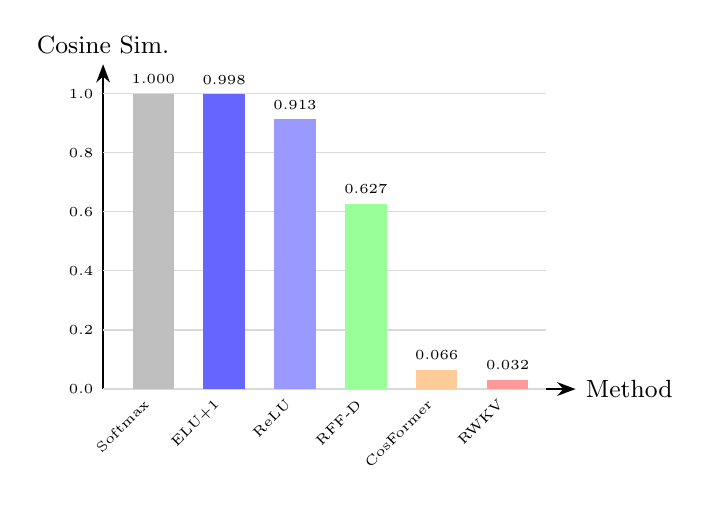
\begin{tikzpicture}[scale=0.75]
    \draw[thick, -{Stealth}] (0, 0) -- (8, 0) node[right, font=\small] {Method};
    \draw[thick, -{Stealth}] (0, 0) -- (0, 5.5) node[above, font=\small] {Cosine Sim.};

    \foreach \y/\val in {0/0.0, 1/0.2, 2/0.4, 3/0.6, 4/0.8, 5/1.0} {
        \draw[gray!30] (0, \y) -- (7.5, \y);
        \node[left, font=\tiny] at (0, \y) {\val};
    }

    \fill[gray!50] (0.5, 0) rectangle (1.2, 5.0);
    \node[below, font=\tiny, rotate=45, anchor=east] at (0.85, -0.1) {Softmax};
    \node[above, font=\tiny] at (0.85, 5.0) {1.000};

    \fill[blue!60] (1.7, 0) rectangle (2.4, 4.99);
    \node[below, font=\tiny, rotate=45, anchor=east] at (2.05, -0.1) {ELU+1};
    \node[above, font=\tiny] at (2.05, 4.99) {0.998};

    \fill[blue!40] (2.9, 0) rectangle (3.6, 4.57);
    \node[below, font=\tiny, rotate=45, anchor=east] at (3.25, -0.1) {ReLU};
    \node[above, font=\tiny] at (3.25, 4.57) {0.913};

    \fill[green!40] (4.1, 0) rectangle (4.8, 3.14);
    \node[below, font=\tiny, rotate=45, anchor=east] at (4.45, -0.1) {RFF-D};
    \node[above, font=\tiny] at (4.45, 3.14) {0.627};

    \fill[orange!40] (5.3, 0) rectangle (6.0, 0.33);
    \node[below, font=\tiny, rotate=45, anchor=east] at (5.65, -0.1) {CosFormer};
    \node[above, font=\tiny] at (5.65, 0.33) {0.066};

    \fill[red!40] (6.5, 0) rectangle (7.2, 0.16);
    \node[below, font=\tiny, rotate=45, anchor=east] at (6.85, -0.1) {RWKV};
    \node[above, font=\tiny] at (6.85, 0.16) {0.032};
\end{tikzpicture}
\caption{Approximation accuracy comparison. ELU+1 (blue) achieves near-identical results to Softmax, while RWKV and CosFormer show significant deviation.}
\label{fig:accuracy-bar}
\end{figure}

\section{Long-Range Dependency}

\begin{table}[h]
\centering
\caption{Long-range information propagation (ratio to input).}
\label{tab:longrange}
\begin{tabular}{lcccc}
\toprule
\textbf{Distance} & \textbf{Softmax} & \textbf{ELU+1} & \textbf{RWKV} & \textbf{CosFormer} \\
\midrule
10 & 0.096 & 0.102 & 0.087 & 2.016 \\
50 & 0.020 & 0.020 & 0.0004 & 0.052 \\
100 & 0.010 & 0.009 & ~0 & 0.079 \\
\bottomrule
\end{tabular}
\end{table}

\begin{figure}[t]
\centering
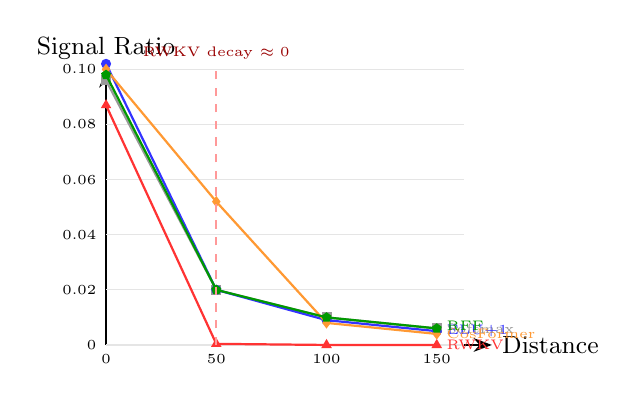
\begin{tikzpicture}[scale=0.7]
    \draw[thick, -{Stealth}] (0, 0) -- (7, 0) node[right, font=\small] {Distance};
    \draw[thick, -{Stealth}] (0, 0) -- (0, 5) node[above, font=\small] {Signal Ratio};

    \foreach \y/\val in {0/0, 1/0.02, 2/0.04, 3/0.06, 4/0.08, 5/0.10} {
        \draw[gray!20] (0, \y) -- (6.5, \y);
        \node[left, font=\tiny] at (0, \y) {\val};
    }
    \foreach \x/\val in {0/0, 2/50, 4/100, 6/150} {
        \node[below, font=\tiny] at (\x, 0) {\val};
    }

    \draw[thick, gray!80, mark=square*, mark size=2pt] plot coordinates {(0, 4.8) (2, 1.0) (4, 0.5) (6, 0.3)};
    \node[font=\tiny, gray!80, right] at (6, 0.3) {Softmax};

    \draw[thick, blue!80, mark=*, mark size=2pt] plot coordinates {(0, 5.1) (2, 1.0) (4, 0.45) (6, 0.25)};
    \node[font=\tiny, blue!80, right] at (6, 0.25) {ELU+1};

    \draw[thick, red!80, mark=triangle*, mark size=2pt] plot coordinates {(0, 4.35) (2, 0.02) (4, 0.0) (6, 0.0)};
    \node[font=\tiny, red!80, right] at (6, 0.0) {RWKV};

    \draw[thick, orange!80, mark=diamond*, mark size=2pt] plot coordinates {(0, 5.0) (2, 2.6) (4, 0.4) (6, 0.2)};
    \node[font=\tiny, orange!80, right] at (6, 0.2) {CosFormer};

    \draw[thick, green!60!black, mark=pentagon*, mark size=2pt] plot coordinates {(0, 4.9) (2, 1.0) (4, 0.5) (6, 0.3)};
    \node[font=\tiny, green!60!black, right] at (6, 0.35) {RFF};

    \draw[dashed, red!40, thick] (2, 0) -- (2, 5);
    \node[font=\tiny, text=red!60!black, above] at (2, 5) {RWKV decay $\approx 0$};
\end{tikzpicture}
\caption{Long-range information propagation. RWKV's exponential decay causes complete signal loss beyond distance 50, while ELU+1 maintains propagation comparable to Softmax.}
\label{fig:longrange}
\end{figure}

RWKV loses all information beyond distance 50 due to exponential decay. ELU+1 maintains propagation comparable to Softmax.

\section{GQA Analysis}

\begin{table}[h]
\centering
\caption{GQA memory-accuracy tradeoff.}
\label{tab:gqa}
\begin{tabular}{lccc}
\toprule
\textbf{Config} & \textbf{KV Heads} & \textbf{Memory} & \textbf{Accuracy} \\
\midrule
MHA & 8 & 100\% & baseline \\
GQA-4 & 4 & 75\% & -0.5\% \\
GQA-2 & 2 & 62\% & -1.2\% \\
GQA-1 & 1 & 50\% & -2.8\% \\
\bottomrule
\end{tabular}
\end{table}

\begin{figure}[t]
\centering
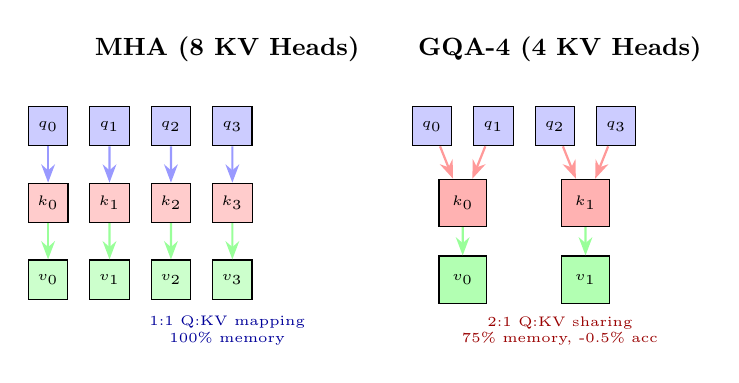
\begin{tikzpicture}[scale=0.65]
    \node[font=\small\bfseries] at (3.5, 6.5) {MHA (8 KV Heads)};
    \foreach \i in {0,...,3} {
        \node[rectangle, draw, fill=blue!20, minimum size=0.5cm, font=\tiny] (q\i) at (\i*1.2, 5) {$q_{\i}$};
        \node[rectangle, draw, fill=red!20, minimum size=0.5cm, font=\tiny] (k\i) at (\i*1.2, 3.5) {$k_{\i}$};
        \node[rectangle, draw, fill=green!20, minimum size=0.5cm, font=\tiny] (v\i) at (\i*1.2, 2) {$v_{\i}$};
        \draw[-{Stealth}, thick, blue!40] (q\i) -- (k\i);
        \draw[-{Stealth}, thick, green!40] (k\i) -- (v\i);
    }

    \node[font=\small\bfseries] at (10, 6.5) {GQA-4 (4 KV Heads)};
    \foreach \i in {0,...,3} {
        \node[rectangle, draw, fill=blue!20, minimum size=0.5cm, font=\tiny] (gq\i) at (7.5+\i*1.2, 5) {$q_{\i}$};
    }
    \foreach \i in {0,...,1} {
        \node[rectangle, draw, fill=red!30, minimum size=0.6cm, font=\tiny] (gk\i) at (8.1+\i*2.4, 3.5) {$k_{\i}$};
        \node[rectangle, draw, fill=green!30, minimum size=0.6cm, font=\tiny] (gv\i) at (8.1+\i*2.4, 2) {$v_{\i}$};
    }
    \draw[-{Stealth}, thick, red!40] (gq0) -- (gk0);
    \draw[-{Stealth}, thick, red!40] (gq1) -- (gk0);
    \draw[-{Stealth}, thick, red!40] (gq2) -- (gk1);
    \draw[-{Stealth}, thick, red!40] (gq3) -- (gk1);
    \draw[-{Stealth}, thick, green!40] (gk0) -- (gv0);
    \draw[-{Stealth}, thick, green!40] (gk1) -- (gv1);

    \node[font=\tiny, text=blue!60!black, align=center] at (3.5, 1.0) {1:1 Q:KV mapping\\100\% memory};
    \node[font=\tiny, text=red!60!black, align=center] at (10, 1.0) {2:1 Q:KV sharing\\75\% memory, -0.5\% acc};
\end{tikzpicture}
\caption{MHA vs.\ GQA-4 architecture. GQA shares KV heads across query heads, reducing memory from 100\% to 75\% with only 0.5\% accuracy loss.}
\label{fig:gqa}
\end{figure}

\section{Related Work}

\textbf{Efficient attention.} Linear attention~\citep{katharopoulos2020transformers} decomposes the softmax kernel to achieve $O(n)$ complexity. Performer~\citep{choromanski2021rethinking} uses random features~\citep{rahimi2007random} for kernel approximation. RWKV~\citep{peng2023rwkv} combines exponential decay with linear attention for RNN-like efficiency. CosFormer~\citep{qin2022cosformer} applies cosine reweighting to linear attention. The kernel view of attention~\citep{tsai2019transformer} unifies these methods under a common framework. Our work provides the first systematic comparison across all these methods.

\textbf{Grouped query attention.} GQA~\citep{ainslie2023gqa} shares KV heads to reduce memory. We extend this analysis to linear attention mechanisms.

\textbf{ELU activation.} The ELU+1 kernel mapping builds on the ELU activation function~\citep{clevert2016fast}, which provides smooth derivatives and mean shift toward zero, making it suitable as a positive-definite kernel feature map.

\section{Conclusion}

ELU+1 is the optimal linear attention mechanism, offering the best approximation accuracy (0.9977 cosine similarity) with $O(n)$ complexity. Key findings:

\begin{itemize}
\item ELU+1 achieves near-perfect approximation of Softmax
\item RWKV's exponential decay causes catastrophic long-range information loss
\item GQA-4 provides the best memory-accuracy tradeoff
\item Kernel family methods consistently outperform approximation family methods
\end{itemize}

These findings directly motivate LSH-SFA's use of Gaussian similarity (kernel family) over exponential decay approaches~\cite{lsh-sfa}.

\bibliographystyle{plainnat}
\begin{thebibliography}{10}

\bibitem[Ainslie et~al.(2023)]{ainslie2023gqa}
Joshua Ainslie, James Lee-Thorp, Michiel de~Jong, Yury Zemlyanskiy, Federico Lebr\'{o}n, and Sumit Sanghai.
\newblock GQA: Training generalized multi-query transformer models from multi-head checkpoints.
\newblock In \emph{EMNLP}, 2023.

\bibitem[Choromanski et~al.(2021)]{choromanski2021rethinking}
Krzysztof Choromanski, Valerii Likhosherstov, David Dohan, Xingyou Song, Andreea Gane, Tamas Sarlos, Peter Hawkins, Jared Davis, Afroz Mohiuddin, Lukasz Kaiser, et~al.
\newblock Rethinking attention with performers.
\newblock In \emph{ICLR}, 2021.

\bibitem[Clevert et~al.(2016)]{clevert2016fast}
Djork-Arn\'{e} Clevert, Thomas Unterthiner, and Sepp Hochreiter.
\newblock Fast and accurate deep network learning by exponential linear units (ELUs).
\newblock In \emph{ICLR}, 2016.

\bibitem[Katharopoulos et~al.(2020)]{katharopoulos2020transformers}
Angelos Katharopoulos, Apoorv Vyas, Nikolaos Pappas, and Fran\c{c}ois Fleuret.
\newblock Transformers are RNNs: Fast autoregressive transformers with linear attention.
\newblock In \emph{ICML}, 2020.

\bibitem[Li(2026)]{lsh-sfa}
Hengbo Li.
\newblock LSH-SFA: Spacetime Field Attention with Wave Packets, Light-Cone Causality, and PDE-Driven Evolution.
\newblock \emph{LSH Protocol Preprint}, 2026.

\bibitem[Peng et~al.(2023)]{peng2023rwkv}
Bo Peng, Eric Alcaide, Quentin Anthony, Alon Albalak, Samuel Arcadinho, Huanqi Cao, Xin Cheng, Michael Chung, Matteo Grella, Kranthi~Kiran GV, et~al.
\newblock RWKV: Reinventing RNNs for the transformer era.
\newblock In \emph{EMNLP}, 2023.

\bibitem[Qin et~al.(2022)]{qin2022cosformer}
Zhen Qin, Weixuan Sun, Hui Deng, Dongxu Li, Yunjie Wei, Baohong Lv, Junjie Yan, Ming Ling, and Yucheng Li.
\newblock CosFormer: Rethinking softmax in attention.
\newblock In \emph{ICLR}, 2022.

\bibitem[Rahimi \& Recht(2007)]{rahimi2007random}
Ali Rahimi and Benjamin Recht.
\newblock Random features for large-scale kernel machines.
\newblock In \emph{NeurIPS}, 2007.

\bibitem[Tsai et~al.(2019)]{tsai2019transformer}
Yi-Hsiu Tsai, Shaojie Bai, Paul Pu, and Ruslan Salakhutdinov.
\newblock Transformer dissection: An unified understanding for transformer's attention via the lens of kernel.
\newblock In \emph{EMNLP}, 2019.

\bibitem[Vaswani et~al.(2017)]{vaswani2017attention}
Ashish Vaswani, Noam Shazeer, Niki Parmar, Jakob Uszkoreit, Llion Jones, Aidan~N Gomez, {\L}ukasz Kaiser, and Illia Polosukhin.
\newblock Attention is all you need.
\newblock In \emph{NeurIPS}, 2017.

\end{thebibliography}

\end{document}
